\documentclass{airep}
\title{
    \large \color{maintheme!70!black} 机器学习项目报告\par\vspace{10pt}
    \color{maintheme!70!black}\bfseries\Large 基于 CNN 与 RNN 结合的草图分类网络  % TBD
}
\author{\kaishu 李子龙~~唐 珂~~裴禹乔}
\date{\today}
\addbibresource{ref.bib}
\begin{document}
\maketitle
\begin{abstract}
本项目旨在解决 25 类草图图像分类问题。首先采用 CNN 网络(Sketch-a-Net, AlexNet, ResNet)对光栅化后的图像利用其局部信息进行识别,之后采用 RNN 的双向 LSTM 结构对笔画利用其顺序信息进行分类,最终使用 CNN 网络(Sketch-a-Net)与 RNN 网络(BiLSTM)相结合的方法得到了较好的分类结果。
\end{abstract}
\section{Introduction}
徒手素描是人类历史上传达信息和表达情感的一种有效方式。素描草图不仅包含目标对象生动的分类特征,而且还包含抽象、多样的视觉表现。在本项目中,我们需要针对大小为 $28\times 28$ 的 25 类 草图图像(如图 \ref{fig:cate} 所示)构建深度学习模型以达到较好的分类效果,并对不同的网络结构性能进行比较。

\begin{figure}[ht]
    \centering
    \includegraphics[width=7cm]{img/sketches.png}
    \caption{25个类别的草图}
    \label{fig:cate}
\end{figure}
\section{Main Ideas}
本小组首先尝试从图像入手,搭建并训练了多种CNN网络对图像进行分类并观察其分类结果。考虑到图像由相应的笔画序列生成,我们后续尝试了通过RNN架构直接对笔画序列进行分类。最终我们将二者结合,通过CNN+RNN的方式结合图像信息和笔画序列信息对图片进行分类。

\begin{figure}[ht]
    \centering
    \scalebox{0.7}{
          \begin{tikzpicture}[mindmap,concept color=gray!50!blue]
      \node [concept] {\color{white}CNN+RNN}
      child[concept color=blue!75,grow=150] {
      	node[concept] {\color{white}CNN} 
      		child[concept color=blue!40,grow=140] {node[concept] {Sketch-a-Net}}
      		child[concept color=blue!40,grow=180] {node[concept] {AlexNet}}
      		child[concept color=blue!40,grow=220] {node[concept] {ResNet}}
      }
      child[concept color=gray,grow=210] {
      	node[concept] {\color{white}RNN}
      		child[concept color=gray!60,grow=180] {node[concept] {BiLSTM}}
      };
      \end{tikzpicture}
    
    }
    \caption{思维导图}
    \label{fig:mindmap}
\end{figure}
\section{Methods and algorithms}\label{sec:methods}
\subsection{数据集预处理}
QuickDraw数据集\cite{sketchrnn}由数百个常见涂鸦对象类组成。每个QuickDraw对象类数据集包含70000个训练样本以及2500个验证样本。QuickDraw使用了一种数据格式,将草图表示为一组笔画动作,该格式中将 0/1 笔画事件扩展为多状态事件。在此数据格式中,图形的初始绝对坐标位于原点,并将草图表示为由点构成的列表,每个点表示为由5个元素组成的向量:$(\Delta x, \Delta y, p_1, p_2, p_3)$。
其中前两个元素是笔划在 $x$ 和 $y$ 方向上相对于前一点的偏移距离,后三个元素表示当前画笔的三种可能状态。第一个笔状态 $p_1$ 表示笔当前正在接触纸张,并且将绘制一条线,将下一点与当前点连接起来。第二个笔状态 $p_2$ 表示笔将在当前点之后从纸上提起,下一步不会画线。第三个笔状态 $p_3$ 表示图形已结束,后续点(包括当前点)将不会渲染。

由于我们使用的 QuickDraw 数据集中的原始草图是以矢量化序列呈现的,为使用基于图片的 CNN 网络架构我们需要首先将其进一步转化为草图图像。为此我们参考了 \parencite{pix2seq} 提供的通过矢量化序列创建草图图像的方法,将 QuickDraw 数据集的笔画格式首先转换为 SVG 图像,后转化为相应的图片形式,如图 \ref{fig:seq2png} 所示。

\begin{figure}[ht]
    \centering
    
      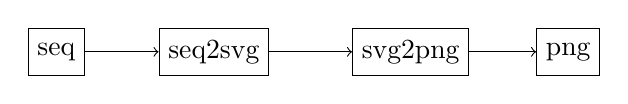
\begin{tikzpicture}[every node/.style={minimum height=0.6cm}]
      \node[draw] (v1) at (0.5,-0.5) {seq};
\node[draw] (v2) at (2.5,-0.5) {seq2svg};
\node[draw] (v3) at (5,-0.5) {svg2png};
\node[draw] (v4) at (7,-0.5) {png};
\draw[->]  (v1) edge (v2);
\draw[->]  (v2) edge (v3);
\draw[->]  (v3) edge (v4);
\end{tikzpicture}
    
    \caption{将笔画格式转换为图像}
    \label{fig:seq2png}
\end{figure}


%%%%% 这段没用到
% RPCL-pix2seq构造了一个分
% 层结构的网络,将底层网络参数和顶层 GMM 参数
% 的训练过程分离,顶层通过RPCL的EM算法估计 GMM 参数,底层通过网络
% 优化器更新网络参数。此外,通过竞争惩罚竞争学习(RPCL)策略的增强,RPCL-pix2seq能够自动确定 GMM
% 的高斯成分数量,从而使可控合成具有更好的鲁棒性。
\subsection{CNN}

\subsubsection{动机}
首先我们尝试以图片作为数据集,因此选择了适用于图像处理的CNN网络结构。卷积神经网络(CNN)主要是用于图像识别领域,CNN的结构通常可以分为3层:
卷积层(Convolutional Layer) --- 主要作用是提取特征;
池化层(Max Pooling Layer) --- 主要作用是下采样(downsampling),却不会损坏识别结果;
全连接层(Fully Connected Layer) --- 主要作用是进行分类。
在图像数据集上使用CNN网络通常可以取得较好的分类结果,为此我们分别使用了代表性的Sketch-a-Net、AlexNet、ResNet-18网络架构,选择QuickDraw图片数据集作为我们的训练集,并在测试集对不同网络架构的分类准确性进行了测试。

\subsubsection{Sketch-a-Net}

Sketch-a-Net\cite{sketchanet}是Qian Yu等人针对手绘草图识别问题提出的多通道的深度神经网络框架,Sketch-a-Net使得计算机对手绘草图的识别能力首次超过了人类。
% Sketch-a-Net通过多通道的方式增加了对绘图过程中不同的绘制顺序的考虑,并通过贝叶斯融合的手段对多尺度的网络进行了融合,从而可以有效解决手绘草图不同程度的提取和稀疏问题。
同时,Sketch-a-Net使用了15×15的卷积核,由于手绘草图缺少纹理信息,较大的卷积核可以更好的体现草图的结构信息。我们复现了其代码,并在其基础上将训练数据集修改为QuickDraw数据集。

\begin{figure}[htp]
    \centering
    \scalebox{1.5}{
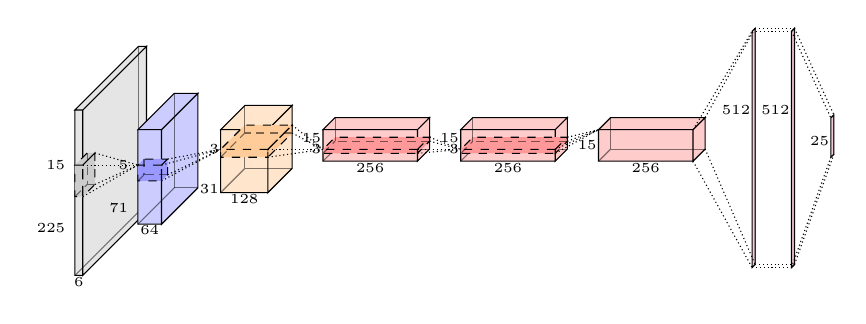
\begin{tikzpicture}
  \tikzset{
    annotated cuboid/.pic={
      \tikzset{%
        every edge quotes/.append style={midway, auto},
        /cuboid/.cd,
        #1
      }
      \draw [\cubeline,every edge/.append style={pic actions, \cubeback, opacity=.5}, pic actions]
      (0,0,0) coordinate (o-\cubelabel) -- ++(-\cubescale*\cubex,0,0) coordinate (a-\cubelabel) -- ++(0,-\cubescale*\cubey,0) coordinate (b-\cubelabel) edge coordinate [pos=1] (g-\cubelabel) ++(0,0,-\cubescale*\cubez)  -- ++(\cubescale*\cubex,0,0) coordinate (c-\cubelabel) -- cycle
      (o-\cubelabel) -- ++(0,0,-\cubescale*\cubez) coordinate (d-\cubelabel) -- ++(0,-\cubescale*\cubey,0) coordinate (e-\cubelabel) edge (g-\cubelabel) -- (c-\cubelabel) -- cycle
      (o-\cubelabel) -- (a-\cubelabel) -- ++(0,0,-\cubescale*\cubez) coordinate (f-\cubelabel) edge (g-\cubelabel) -- (d-\cubelabel) -- cycle;
      ;
    },
    /cuboid/.search also={/tikz},
    /cuboid/.cd,
    width/.store in=\cubex,
    height/.store in=\cubey,
    depth/.store in=\cubez,
    units/.store in=\cubeunits,
    scale/.store in=\cubescale,
    label/.store in=\cubelabel,
    line/.store in=\cubeline,
    backline/.store in=\cubeback,
    width=10,
    height=10,
    depth=10,
    units=cm,
    scale=.1,
    line=draw,
    backline=densely dashed,
    font=\tiny
  }
  
  \pic [fill=gray!20, text=green!50!black, draw=black] at (4,-2) {annotated cuboid={label=A, width=1, height=21, depth=21, units=mm, backline=draw}};

  \node [left,yshift=-1.5cm] at (a-A) {225};
  \node [below,xshift=0.05cm,yshift=0.1cm] at (b-A) {6};

  \pic [fill=gray!40, text=green!50!black, draw=black] at (4,-2.7) {annotated cuboid={label=B, width=1, height=4, depth=4, units=m, line=dashed}};

  \node [left] at (a-B) {15};

  \pic [fill=blue!20, text=green!50!black, draw=black] at (5,-2.25) {annotated cuboid={label=C, width=3, height=12, depth=12, units=mm, backline=draw}};
	
  \node [left,yshift=-1cm] at (a-C) {71};
  \node [below,xshift=0.15cm,yshift=0.1cm] at (b-C) {64};

  \pic [fill=blue!40, text=green!50!black, draw=black] at (5,-2.7) {annotated cuboid={label=D, width=3, height=2, depth=2, units=m, line=dashed}};

  \node [left] at (a-D) {5};

  \pic [fill=orange!20, text=green!50!black, draw=black] at (6.35,-2.25) {annotated cuboid={label=E, width=6, height=8, depth=8, units=m, backline=draw}};

  \node [left,xshift=0.1cm,yshift=-0.75cm] at (a-E) {31};
  \node [below,xshift=0.3cm,yshift=0.1cm] at (b-E) {128};

  \pic [fill=orange!40, text=green!50!black, draw=black] at (6.35,-2.5) {annotated cuboid={label=F, width=6, height=1, depth=8, units=m, line=dashed}};

  \node [left,xshift=0.1cm] at (a-F) {3};

  \pic [fill=red!20, text=green!50!black, draw=black] at (8.25,-2.25) {annotated cuboid={label=G, width=12, height=4, depth=4, units=m, backline=draw}};

  \node [left,xshift=0.1cm,yshift=-0.1cm] at (a-G) {15};
  \node [below,xshift=0.6cm,yshift=0.1cm] at (b-G) {256};

  \pic [fill=red!40, text=green!50!black, draw=black] at (8.25,-2.5) {annotated cuboid={label=H, width=12, height=0.5, depth=4, units=m, line=dashed}};

  \node [left,xshift=0.1cm] at (a-H) {3};

  \pic [fill=red!20, text=green!50!black, draw=black] at (10,-2.25) {annotated cuboid={label=I, width=12, height=4, depth=4, units=m, backline=draw}};

  \node [left,xshift=0.1cm,yshift=-0.1cm] at (a-I) {15};
  \node [below,xshift=0.6cm,yshift=0.1cm] at (b-I) {256};

  \pic [fill=red!40, text=green!50!black, draw=black] at (10,-2.5) {annotated cuboid={label=J, width=12, height=0.5, depth=4, units=m, line=dashed}};

  \node [left,xshift=0.1cm] at (a-J) {3};

  \pic [fill=red!20, text=green!50!black, draw=black] at (11.75,-2.25) {annotated cuboid={label=K, width=12, height=4, depth=4, units=m, backline=draw}};
  
  \node [left,xshift=0.1cm,yshift=-0.2cm] at (a-K) {15};
  \node [below,xshift=0.6cm,yshift=0.1cm] at (b-K) {256};

  
  \pic [fill=purple!20, text=green!50!black, draw=black] at (12.5,-1) {annotated cuboid={label=L, width=0, height=30, depth=1, units=m, backline=draw}};

  \node [left,xshift=0.1cm,yshift=-1cm] at (a-L) {512};

  \pic [fill=purple!20, text=green!50!black, draw=black] at (13,-1) {annotated cuboid={label=M, width=0, height=30, depth=1, units=m, backline=draw}};

  \node [left,xshift=0.1cm,yshift=-1cm] at (a-M) {512};  

  \pic [fill=purple!20, text=green!50!black, draw=black] at (13.5,-2.1) {annotated cuboid={label=N, width=0, height=5, depth=1, units=m, backline=draw}};

  \node [left,xshift=0.1cm,yshift=-0.3cm] at (a-N) {25}; 

  \foreach \point in {c,d,e,o} {
    \draw[densely dotted] (\point-B) -- (a-D);
    \draw[densely dotted] (\point-D) -- (a-F);
    \draw[densely dotted] (\point-F) -- (a-H);
    \draw[densely dotted] (\point-H) -- (a-J);
  	\draw[densely dotted] (\point-J) -- (a-K);
  	\draw[densely dotted] (\point-K) -- (\point-L);
    \draw[densely dotted] (\point-L) -- (\point-M);
    \draw[densely dotted] (\point-M) -- (\point-N);
  }
\end{tikzpicture}
}
    \caption{Sketch-a-Net结构}
    \label{fig:sketch-a-net}
\end{figure}
\subsubsection{AlexNet}
AlexNet\cite{alexnet}卷积神经网络模型由5个卷积层和3个池化Pooling层以及3个全连接层构成,如图 \ref{fig:Alexnet} 所示。其特点在于:使用ReLU作为CNN的激活函数,ReLU函数的效果在较深的网络中超过常规的Sigmoid函数,解决了Sigmoid在网络较深时的梯度弥散问题;在训练时使用Dropout随机忽略一部分神经元,以避免模型过拟合;并且在CNN中使用重叠的最大池化(步长小于卷积核),此前CNN中普遍使用平均池化,使用最大池化可以避免平均池化的模糊效果,同时重叠效果可以提升特征的丰富性;并且AlexNet使用了LRN层(Local Response Normalization,即局部响应归一化),对局部神经元的活动创建竞争机制,使得其中响应比较大的值变得相对更大,并抑制其他反馈较小的神经元,增强了模型的泛化能力。在AlexNet的基础上我们将QuickDraw数据集中28×28的图片resize为225×225进而作为AlexNet的输入,最终通过训练得到了较好的分类结果。
\begin{figure}[htp]
    \centering
    \includegraphics[width=15cm]{img/alexnet.pdf}
    % {
    % 
\def\ConvColor{rgb:yellow,5;red,2.5;white,5}
\def\ConvReluColor{rgb:yellow,5;red,5;white,5}
\def\PoolColor{rgb:red,1;black,0.3}
\def\UnpoolColor{rgb:blue,2;green,1;black,0.3}
\def\FcColor{rgb:blue,2;green,5;white,5}
\def\FcReluColor{blue,2;green,5;;white,4}
\def\SoftmaxColor{rgb:magenta,5;black,7}   

\def\edgecolor{rgb:blue,4;red,1;green,4;black,3}
\newcommand{\midarrow}{\tikz \draw[-Stealth,line width =0.8mm,draw=\edgecolor] (-0.3,0) -- ++(0.3,0);}

\tikzset{Box/.pic={\tikzset{/boxblock/.cd,#1}
        \tikzstyle{box}=[every edge/.append style={pic actions, densely dashed, opacity=.7},fill opacity=\opacity, pic actions,fill=\fill]
        
        \pgfmathsetmacro{\y}{\cubey*\scale}
        \pgfmathsetmacro{\z}{\cubez*\scale}
   
        %Multiple concatenated boxes
        \foreach[count=\i,%
                 evaluate=\i as \xlabel using {array({\boxlabels},\i-1)},% 
                 evaluate=\unscaledx as \k using {\unscaledx*\scale+\prev}, remember=\k as \prev (initially 0)] 
                 \unscaledx in \cubex
        {
            \pgfmathsetmacro{\x}{\unscaledx*\scale}
            \coordinate (a) at (\k-\x , \y/2 , \z/2); 
            \coordinate (b) at (\k-\x ,-\y/2 , \z/2); 
            \coordinate (c) at (\k    ,-\y/2 , \z/2); 
            \coordinate (d) at (\k    , \y/2 , \z/2); 
            \coordinate (e) at (\k    , \y/2 ,-\z/2); 
            \coordinate (f) at (\k    ,-\y/2 ,-\z/2); 
            \coordinate (g) at (\k-\x ,-\y/2 ,-\z/2); 
            \coordinate (h) at (\k-\x , \y/2 ,-\z/2); 
        
            \draw [box] 
                (d) -- (a) -- (b) -- (c) -- cycle     
                (d) -- (a) -- (h) -- (e) -- cycle
                %dotted edges
                (f) edge (g)
                (b) edge (g)
                (h) edge (g)    
            ;
            \path (b) edge ["\xlabel"',midway] (c);
            
            \xdef\LastEastx{\k} %\k persists as \LastEastx after loop 
        }%Loop ends
        \draw [box] (d) -- (e) -- (f) -- (c) -- cycle; %East face of last box     
        
        \coordinate (a1) at (0 , \y/2 , \z/2);
        \coordinate (b1) at (0 ,-\y/2 , \z/2);
        \tikzstyle{depthlabel}=[pos=0,text width=14*\z,text centered,sloped]       
        
        \path (c) edge ["\small\zlabel"',depthlabel](f); %depth label
        \path (b1) edge ["\ylabel",midway] (a1);  %height label
        
        
        \tikzstyle{captionlabel}=[text width=15*\LastEastx/\scale,text centered]       
        \path (\LastEastx/2,-\y/2,+\z/2) + (0,-25pt) coordinate (cap) 
        edge ["\textcolor{black}{ \bf \caption}"',captionlabel](cap) ; %Block caption/pic object label
         
        %Define nodes to be used outside on the pic object
        \coordinate (\name-west)   at (0,0,0) ;
        \coordinate (\name-east)   at (\LastEastx, 0,0) ;
        \coordinate (\name-north)  at (\LastEastx/2,\y/2,0);
        \coordinate (\name-south)  at (\LastEastx/2,-\y/2,0);       
        \coordinate (\name-anchor) at (\LastEastx/2, 0,0) ;
        
        \coordinate (\name-near) at (\LastEastx/2,0,\z/2);
        \coordinate (\name-far)  at (\LastEastx/2,0,-\z/2);       
        
        \coordinate (\name-nearwest) at (0,0,\z/2);
        \coordinate (\name-neareast) at (\LastEastx,0,\z/2);
        \coordinate (\name-farwest)  at (0,0,-\z/2);
        \coordinate (\name-fareast)  at (\LastEastx,0,-\z/2);
        
        \coordinate (\name-northeast) at (\name-north-|\name-east);
        \coordinate (\name-northwest) at (\name-north-|\name-west);
        \coordinate (\name-southeast) at (\name-south-|\name-east);
        \coordinate (\name-southwest) at (\name-south-|\name-west);
        
        \coordinate (\name-nearnortheast)  at (\LastEastx, \y/2, \z/2);
        \coordinate (\name-farnortheast)   at (\LastEastx, \y/2,-\z/2);
        \coordinate (\name-nearsoutheast)  at (\LastEastx,-\y/2, \z/2);
        \coordinate (\name-farsoutheast)   at (\LastEastx,-\y/2,-\z/2);
        
        \coordinate (\name-nearnorthwest)  at (0, \y/2, \z/2);
        \coordinate (\name-farnorthwest)   at (0, \y/2,-\z/2);
        \coordinate (\name-nearsouthwest)  at (0,-\y/2, \z/2);
        \coordinate (\name-farsouthwest)   at (0,-\y/2,-\z/2);
        
    },
    /boxblock/.search also={/tikz},
    /boxblock/.cd,
    width/.store        in=\cubex,
    height/.store       in=\cubey,
    depth/.store        in=\cubez,
    scale/.store        in=\scale,
    xlabel/.store       in=\boxlabels,
    ylabel/.store       in=\ylabel,
    zlabel/.store       in=\zlabel,
    caption/.store      in=\caption,
    name/.store         in=\name,
    fill/.store         in=\fill,
    opacity/.store      in=\opacity,
    fill={rgb:red,5;green,5;blue,5;white,15},
    opacity=0.4,
    width=2,
    height=13,
    depth=15,
    scale=.2,
    xlabel={{"","","","","","","","","",""}},
    ylabel=,
    zlabel=,
    caption=,
    name=,
}


\newcommand{\copymidarrow}{\tikz \draw[-Stealth,line width=0.8mm,draw={rgb:blue,4;red,1;green,1;black,3}] (-0.3,0) -- ++(0.3,0);}

\scalebox{0.5}{
\begin{tikzpicture}
\tikzstyle{connection}=[ultra thick,every node/.style={sloped,allow upside down},draw=\edgecolor,opacity=0.7]
\tikzstyle{copyconnection}=[ultra thick,every node/.style={sloped,allow upside down},draw={rgb:blue,4;red,1;green,1;black,3},opacity=0.7]


\pic[shift={(0,0,0)}] at (0,0,0) 
    {Box={
        name=conv0,
        caption= ,
        xlabel={{3, }},
        zlabel=225,
        fill=\ConvColor,
        height=44.8,
        width=3,
        depth=44.8
        }
    };


\pic[shift={(1,0,0)}] at (conv0-east) 
    {Box={
        name=conv1,
        caption= ,
        xlabel={{96, }},
        zlabel=55,
        fill=\ConvColor,
        height=11.0,
        width=4.8,
        depth=11.0
        }
    };


\draw [connection]  (conv0-east)    -- node {\midarrow} (conv1-west);


\pic[shift={ (0,0,0) }] at (conv1-east) 
    {Box={
        name=pool1,
        caption= ,
        fill=\PoolColor,
        opacity=0.5,
        height=5.4,
        width=1,
        depth=5.4
        }
    };


\pic[shift={(1,0,0)}] at (pool1-east) 
    {Box={
        name=conv2,
        caption= ,
        xlabel={{256, }},
        zlabel=27,
        fill=\ConvColor,
        height=5.4,
        width=12.8,
        depth=5.4
        }
    };


\draw [connection]  (pool1-east)    -- node {\midarrow} (conv2-west);


\pic[shift={ (0,0,0) }] at (conv2-east) 
    {Box={
        name=pool2,
        caption= ,
        fill=\PoolColor,
        opacity=0.5,
        height=2.6,
        width=1,
        depth=2.6
        }
    };


\pic[shift={(1,0,0)}] at (pool2-east) 
    {Box={
        name=conv3,
        caption= ,
        xlabel={{384, }},
        zlabel=13,
        fill=\ConvColor,
        height=2.6,
        width=19.2,
        depth=2.6
        }
    };


\draw [connection]  (pool2-east)    -- node {\midarrow} (conv3-west);


\pic[shift={(1,0,0)}] at (conv3-east) 
    {Box={
        name=conv4,
        caption= ,
        xlabel={{384, }},
        zlabel=13,
        fill=\ConvColor,
        height=2.6,
        width=19.2,
        depth=2.6
        }
    };


\draw [connection]  (conv3-east)    -- node {\midarrow} (conv4-west);


\pic[shift={(1,0,0)}] at (conv4-east) 
    {Box={
        name=conv5,
        caption= ,
        xlabel={{256, }},
        zlabel=13,
        fill=\ConvColor,
        height=2.6,
        width=12.8,
        depth=2.6
        }
    };


\draw [connection]  (conv4-east)    -- node {\midarrow} (conv5-west);


\pic[shift={ (0,0,0) }] at (conv5-east) 
    {Box={
        name=pool3,
        caption= ,
        fill=\PoolColor,
        opacity=0.5,
        height=1.2,
        width=1,
        depth=1.2
        }
    };


\pic[shift={(1,0,0)}] at (pool3-east) 
    {Box={
        name=Fc1,
        caption= ,
        xlabel={{1, }},
        zlabel=4096,
        fill=\FcColor,
        height=1,
        width=1,
        depth=40.96
        }
    };


\draw [connection]  (pool3-east)    -- node {\midarrow} (Fc1-west);


\pic[shift={(2,0,0)}] at (Fc1-east) 
    {Box={
        name=Fc2,
        caption= ,
        xlabel={{1, }},
        zlabel=4096,
        fill=\FcColor,
        height=1,
        width=1,
        depth=40.96
        }
    };


\draw [connection]  (Fc1-east)    -- node {\midarrow} (Fc2-west);


\pic[shift={(3,0,0)}] at (Fc2-east) 
    {Box={
        name=soft1,
        caption=SOFT,
        xlabel={{" ","dummy"}},
        zlabel=25,
        fill=\SoftmaxColor,
        opacity=0.8,
        height=3,
        width=1.5,
        depth=25
        }
    };


\draw [connection]  (Fc2-east)    -- node {\midarrow} (soft1-west);


\end{tikzpicture}
}
    % }
    
    \caption{AlexNet结构}
    \label{fig:Alexnet}
\end{figure}
\subsubsection{ResNet-18}
ResNet\cite{resnet}网络参考了VGG19网络,沿用了VGG完整的3×3卷积层设计,并在其基础上通过短路机制加入了残差单元。残差单元里首先有2个有相同输出通道数的3×3卷积层,每个卷积层后接一个批量规范化层和ReLU激活函数,残差单元通过跨层数据通路,跳过这2个卷积运算,将输入直接加在最后的ReLU激活函数中。通过以上方式,ResNet很好的处理了深度卷积网络在图像分类中的退化问题。

\begin{figure}[ht]
    \centering
    \input{img/resnet}
    \caption{ResNet-18结构}
    \label{fig:ResNet-18}
\end{figure}

\subsection{RNN}

\subsubsection{动机}
考虑到原QucikDraw数据集由笔画序列构成,我们尝试了对序列处理较为高效的RNN架构。循环神经网络(RNN),同经典的前馈神经网络相比较(如多层感知器、深度置信网络、卷积神经网络等),RNN允许网络隐藏层(hidden layer)的输出再以输入的形式作用于该隐藏层自己。

由于RNN具有记忆性并且具有参数共享的特征,在对序列的非线性特征进行学习时具有一定优势,而RNN单元在面对长序列数据时,很容易便遭遇梯度弥散,使得RNN只具备短期记忆。

而长短期记忆网络(Long-Short Term Memory, LSTM)通过引入遗忘门(forget gate)、输入门(input gate)、输出门(output gate)等结构控制信息的保留与丢弃,如图 \ref{fig:lstm} 所示。可以有效地解决 RNN 中的梯度爆炸和梯度消失问题,并有效地处理长距离的依赖。

% 对QuickDraw序列数据集进行学习,并取得了较好的结果。LSTM 元胞结构如图 \ref{fig:lstm} 所示。
% RNN 简介

\begin{figure}[ht]
    \centering
    \input{img/lstm}
    \caption{LSTM 元胞结构}
    \label{fig:lstm}
\end{figure}

\subsubsection{双向 LSTM}

SketchRNN \cite{sketchrnn} 采用了可变自编码器(Variational Auto Encoder, VAE)结构生成其他的笔画图像。本项目为分类问题,我们只采用编码器(Encoder)部分的双向 LSTM 结构 \cite{bilstm} 用于分类识别,隐藏层元胞数目为 $256\times 2$,没有对 latent  space 的 $N_z$ 进行生成,而是最后直接添加线性层全连接用于图像的 $25$ 分类。

双向 LSTM 结构(如图 \ref{fig:bilstm})相较于单向的 LSTM 增加了后向传播层,不仅可以考虑之前的状态,还会考虑未来的状态,这样可以更好地识别笔画信息。

% 不仅可以会考虑之前的状态,还会考虑与未来状态的关系。

\begin{figure}[ht]
    \centering
    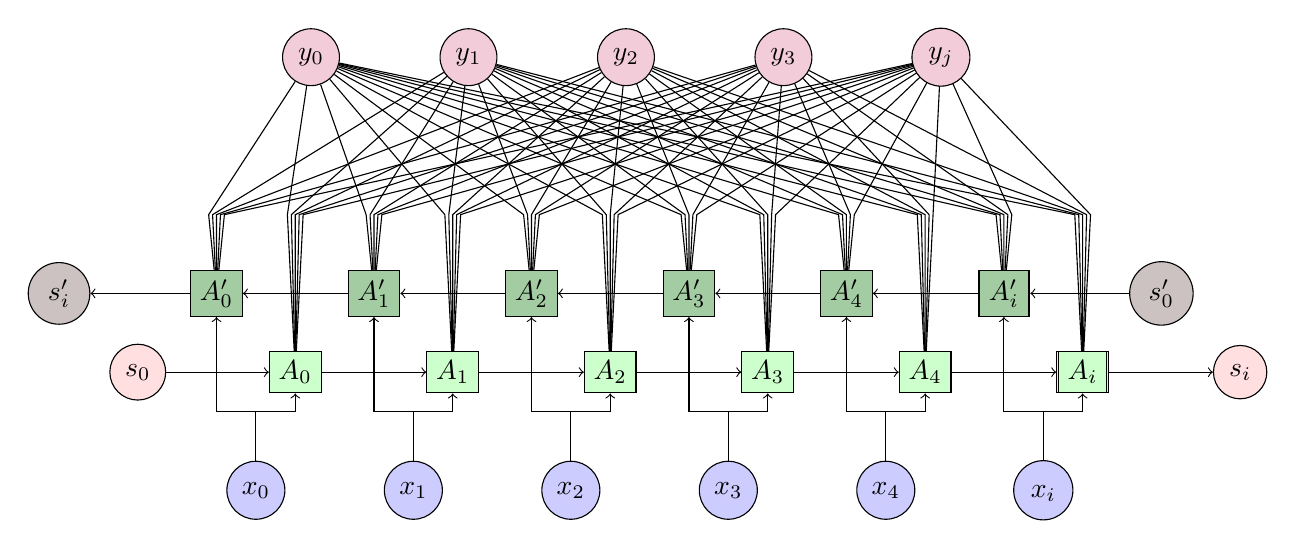
\begin{tikzpicture}
\foreach \i in {0,1,...,5} {
	\node[draw,fill=green!20] (f\i) at (\i*2,0) {$A_\i$};
	\node[draw,fill=green!20!white!80!black] (b\i) at ({(\i-0.5)*2},1) {$A^\prime_\i$};
	\node[draw,circle,fill=blue!20] (x\i) at ({(\i-0.25)*2},-1.5) {$x_\i$};
	%\node[draw,circle] (y\i) at ({(\i-0.25)*2},2.5) {$y_\i$};
	\draw[->] (x\i) -- +(0,1) -| (b\i);
	\draw[->] (x\i) -- +(0,1) -| (f\i);
	%\draw[->] (b\i) -- ++(0,0.5) -- ++(0.5,0) -- (y\i);
	%\draw[->] (f\i) -- ++(0,1.5) -- ++(-0.5,0) -- (y\i);
}
\node[draw,circle,fill=pink!50] (f-1) at (-2,0) {$s_0$};
\node[draw,circle,fill=pink!50] (f6) at (12,0) {$s_i$};
\node[draw,circle,fill=pink!20!white!80!black] (b6) at (11,1) {$s^\prime_0$};
\node[draw,circle,fill=pink!20!white!80!black] (b-1) at (-3,1) {$s^\prime_i$};
\foreach \i in {-1,0,1,...,4,5} {
	\pgfmathparse{int(\i+1)} % int is important
	\draw[->] (f\i) -- (f\pgfmathresult);
	\draw[->] (b\pgfmathresult) -- (b\i);
}
\foreach \j in {0,1,...,4} {
	\node[draw,circle,fill=purple!20] (y\j) at ({(\j+0.1)*2},4) {$y_\j$};
	\foreach \i in {0,...,5} {
		\draw (f\i) -- ++({-0.1+\j*0.05},2) -- (y\j);
		\draw (b\i) -- ++({-0.1+\j*0.05},1) -- (y\j);
	}
}
\node[draw,circle,fill=blue!20] at (9.5,-1.5) {$x_i$\vphantom{1}};
\node[draw,fill=green!20] at (10,0) {$A_i$\vphantom{1}};
\node[draw,fill=green!20!white!80!black] at (9,1) {$A^\prime_i$\vphantom{1}};
\node[draw,fill=purple!20,circle] at (8.2,4) {$y_j$};
\end{tikzpicture}
    \caption{BiLSTM 结构($i=\max{\#seq},j=25$)}
    \label{fig:bilstm}
\end{figure}

\subsection{CNN+RNN}
Peng Xu等人在SketchMate\cite{sketchmate}文章中提出了一种将CNN与RNN结合的网络结构,分别将图片信息输入CNN网络分支并通过CNN提取抽象的视觉概念,将笔画序列信息输入RNN网络分支建模素描的时间顺序,之后再通过后期融合层以及量化编码层将二者进行结合。

我们又参考了 LiveSketch\cite{livesketch} 的网络结构,将 CNN 和 RNN 分支直接连接到全连接层,最后用于分类,如图 \ref{fig:cnnrnn}。其中 CNN 分支使用了 Sketch-a-Net 结构,而 RNN 分支使用了 BiLSTM 结构,全连接层将会同时接收两个分支各 512 个输出(共 1024 个输出)连接于 512 个神经元上,之后全连接于后层用来进行 25 个分类的判别。

\begin{figure}[ht]
    \centering
    \includegraphics{img/cnnrnn.pdf}
    \caption{CNN+RNN 结构(分支各 512 个输出,全连接层 512 个神经元,输出层为 25 分类器)}
    \label{fig:cnnrnn}
\end{figure}



\section{Experimental settings}

\subsection{训练参数}

网络超参数为第 \ref{sec:methods} 节所言的默认参数。训练时参数如表 \ref{tab:param} 所示。

\begin{table}[ht]
    \centering
    \caption{训练参数}
    \label{tab:param}
    \begin{tabular}{cccccc}
        \toprule
        参数 & Sketch-a-Net &  AlexNet & ResNet & BiLSTM & CNN+RNN \\
        \midrule
        lr &  \multicolumn{5}{c}{0.001} \\
        batch size & \multicolumn{5}{c}{64}  \\
        weight decay & 0.001 &  0.001&  0.001& 0.0006  &0.0006 \\
        % \midrule
        % RNN 隐藏层元胞数 & - & - & - & $256\times 2$ & $256\times 2$ \\
        \bottomrule
    \end{tabular}
\end{table}

\subsection{优化训练方法}

\subsubsection{权重衰减}
    权重衰减(weight decay),也可称为L2正则化,其目的是让权重衰减到更小的值,在一定程度上缓解模型过拟合的问题。其之所以有效,是因为L2范数对于权重向量的大分量施加了巨大的惩罚,使学习算法会偏向在大量特征上均匀分布权重的模型,对单个变量上的观测误差更加稳定,而非将权重集中在小部分特征上。
    
    本小组通过设置Adam优化器中 \verb"weight_decay",以抑制模型深度可能过深带来的过拟合现象,增强模型的泛化能力。
\subsubsection{可变的学习率}
    调整学习率也是优化模型十分重要的一环。如果学习率过大,会造成结果难以收敛;而如果学习率太小,既可能导致结果收敛过慢,训练时间过长,也可能导致结果只处于一个局部最优而非更好的结果。因此,在训练的过程当中,我们需要动态衰减学习率。
    
    我们使用了 PyTorch 包中自带的scheduler类来进行学习率衰减,如下面代码所示:
    \begin{lstlisting}
     scheduler = ReduceLROnPlateau(optimizer, 'min', factor=0.3, patience=2)
     train_model(model, dataloaders_dict, criterion, optimizer, scheduler, num_epochs=5)
    \end{lstlisting}
    解释:
    \begin{itemize}
        \item \textbf{patience}:这个参数是容忍程度的意思,意味着在训练数量为patience的轮数之后,如果validation集上的loss一直则没有下降,则要求开始降低学习率。本小组的代码中将这设置成2。
        \item \textbf{factor}:这个参数是学习率衰减时的乘以的因子,本小组将此设置成0.3,意味着每一次衰减为原来的0.3倍。
    \end{itemize}


\section{Experimental results}

% \subsection{训练情况}

训练时验证集准确率的收敛情况如图 \ref{fig:val} 所示。由图可见,CNN 的收敛速度要比 RNN 要快,但是单个批次的训练时间 CNN 会更长一些。在 CNN 中,ResNet 的最终正确率会更高一些。将 CNN 与 RNN 结合的网络最终验证集正确率会比两者单独都要高一些。

\begin{figure}[ht]
    \centering
    \subfigure[CNN]{\includegraphics[width=0.3\textwidth]{img/cnn}}
    \subfigure[RNN]{\includegraphics[width=0.3\textwidth]{img/rnn}}
    \subfigure[CNN+RNN]{\includegraphics[width=0.3\textwidth]{img/cnnrnn.png}}
    \caption{验证集收敛情况}
    \label{fig:val}
\end{figure}

最后将最佳验证准确率对应的网络在 25 个类别所有的测试集进行测试,结果如表 \ref{tab1} 所示。


\begin{table}[H]
\begin{minipage}{0.4\textwidth}
\caption{每一类模型最佳的测试准确率}\label{tab1}
\centering
\begin{tabular}{cc}
\toprule
模型 & 测试准确率 \\
\midrule
Sketch-a-Net & 0.6948\\
AlexNet & 0.8462\\
ResNet18 & 0.8557\\
BiLSTM & 0.8561\\
CNN+RNN & \textbf{0.8567}\\
\bottomrule
\end{tabular}
\end{minipage}
\begin{minipage}{0.55\textwidth}
\centering
\section{Experimental results}

% \subsection{训练情况}

训练时验证集准确率的收敛情况如图 \ref{fig:val} 所示。由图可见,CNN 的收敛速度要比 RNN 要快,但是单个批次的训练时间 CNN 会更长一些。在 CNN 中,ResNet 的最终正确率会更高一些。将 CNN 与 RNN 结合的网络最终验证集正确率会比两者单独都要高一些。

\begin{figure}[ht]
    \centering
    \subfigure[CNN]{\includegraphics[width=0.3\textwidth]{img/cnn}}
    \subfigure[RNN]{\includegraphics[width=0.3\textwidth]{img/rnn}}
    \subfigure[CNN+RNN]{\includegraphics[width=0.3\textwidth]{img/cnnrnn.png}}
    \caption{验证集收敛情况}
    \label{fig:val}
\end{figure}

最后将最佳验证准确率对应的网络在 25 个类别所有的测试集进行测试,结果如表 \ref{tab1} 所示。


\begin{table}[H]
\begin{minipage}{0.4\textwidth}
\caption{每一类模型最佳的测试准确率}\label{tab1}
\centering
\begin{tabular}{cc}
\toprule
模型 & 测试准确率 \\
\midrule
Sketch-a-Net & 0.6948\\
AlexNet & 0.8462\\
ResNet18 & 0.8557\\
BiLSTM & 0.8561\\
CNN+RNN & \textbf{0.8567}\\
\bottomrule
\end{tabular}
\end{minipage}
\begin{minipage}{0.55\textwidth}
\centering
\section{Experimental results}

% \subsection{训练情况}

训练时验证集准确率的收敛情况如图 \ref{fig:val} 所示。由图可见,CNN 的收敛速度要比 RNN 要快,但是单个批次的训练时间 CNN 会更长一些。在 CNN 中,ResNet 的最终正确率会更高一些。将 CNN 与 RNN 结合的网络最终验证集正确率会比两者单独都要高一些。

\begin{figure}[ht]
    \centering
    \subfigure[CNN]{\includegraphics[width=0.3\textwidth]{img/cnn}}
    \subfigure[RNN]{\includegraphics[width=0.3\textwidth]{img/rnn}}
    \subfigure[CNN+RNN]{\includegraphics[width=0.3\textwidth]{img/cnnrnn.png}}
    \caption{验证集收敛情况}
    \label{fig:val}
\end{figure}

最后将最佳验证准确率对应的网络在 25 个类别所有的测试集进行测试,结果如表 \ref{tab1} 所示。


\begin{table}[H]
\begin{minipage}{0.4\textwidth}
\caption{每一类模型最佳的测试准确率}\label{tab1}
\centering
\begin{tabular}{cc}
\toprule
模型 & 测试准确率 \\
\midrule
Sketch-a-Net & 0.6948\\
AlexNet & 0.8462\\
ResNet18 & 0.8557\\
BiLSTM & 0.8561\\
CNN+RNN & \textbf{0.8567}\\
\bottomrule
\end{tabular}
\end{minipage}
\begin{minipage}{0.55\textwidth}
\centering
\input{img/result}
\captionof{figure}{测试准确率统计图}
\end{minipage}
\end{table}


\captionof{figure}{测试准确率统计图}
\end{minipage}
\end{table}


\captionof{figure}{测试准确率统计图}
\end{minipage}
\end{table}


\section{Conclusion}


\subsection{结果分析}

\begin{enumerate}
    \item 从CNN的曲线当中可以看到,验证集的accuracy会随着训练轮数的增加在某一个epoch突然下降,我们猜想这可能跟模型过拟合有关。
    \item 事实上weight\_decay参数对RNN模型的收敛有很大的影响,只有当weight\_decay设置得足够小,比如低于0.001时,RNN的训练才会收敛。这说明仔细调节超参的重要性。
    \item alexnet和resnet18都是在图像识别领域取得巨大成功的模型,在我们的实验中它们的发挥比sketch-a-net要好很多,这说明即使简笔画不同于一般的照片,良好的CNN模型也是有不错的预测能力。但是与正常图片高达95\%以上的预测准确度相比,这些优异的CNN模型在简笔画上的发挥要低上十个百分点,这说明简笔画这种单单仅有几个线条的卡通图片的确会给分类造成困难。
    \item BiLSTM的结果和AlexNet和ResNet18的结果差不多,但是BiLSTM的训练所耗费的资源更少,在给定笔画的情况下,采用这种方法可能会更好。
    \item CNN+RNN上下两路结合的方法在我们的实验当中取得最佳的预测准确度。这种方法同时兼顾了图片的视觉信息以及笔画的序列信息,通过两种神经网路提取出不同维度的feature,并将这两种feature给结合在一起,使得不同的模型可以学习到数据的不同特征,经过融合后的结果往往能有更好的表现,大有取长补短的意思。
\end{enumerate}
\subsection{未来的改进}
\begin{enumerate}
    \item 我们使用RNN的方法是直接将decoder给剔除,然后在encoder最后添加线性层,这种方法可能没有充分使用笔画的序列信息。或许使用VAE,得到每一种种类简笔画背后的latent space能够对分类有很大的帮助。
    \item CNN模型表现不佳可能是因为简笔画不像一般的图片,简笔画中仅仅只有寥寥数笔,其余是大片的空白,如果能够将这些空白给填充起来,或许CNN就能够发挥出更大的威力。
\end{enumerate}

\subsection{小结}

本项目从 CNN 入手,比较了 AlexNet, ResNet, Sketch-A-Net 对图像信息的分类结果,测试结果是 ResNet 略胜一筹。接着使用 RNN 中的双向 LSTM 对笔画数据进行分类,结果略有提升。最后将两者结合起来,最后通过多层神经网络进行分类,结果进一步有所提升。

CNN 优点在于准确率相对较高,收敛速度快。但缺点就是训练时间较长,从笔画转换为图像数据也需要时间。RNN 优点在于训练速度快,但缺点就在于参数不当的情况下,收敛速度会很慢。将两者结合,可以很好地利用图像的局部信息与笔画的产生顺序,更为高效地获得较好的分类模型。

\section*{Contribution}

项目地址:\href{https://github.com/LogCreative/quickdraw-classifier}{https://github.com/LogCreative/quickdraw-classifier}

\begin{table}[h]
    \centering
    \caption{团队贡献}
    \begin{tabular}{clc}
        \toprule
        姓名 & 贡献 & 百分比 \\
        \midrule
        李子龙  & RNN 模型的完善,CNN+RNN 模型的初步构造,报告 & 33.3\% \\
        唐\quad{}珂  & CNN 模型构造,RNN 模型的初步构造,训练模型,报告 & 33.3\% \\
        裴禹乔  &  报告,CNN+RNN 模型的完善 & 33.3\% \\
        \bottomrule
    \end{tabular}
\end{table}

\printbibliography
\end{document}
